\documentclass[a4paper,11pt]{article}
\usepackage[margin=2.4cm]{geometry}
\usepackage{amsmath,amssymb}
\usepackage{booktabs}
\usepackage{multirow}
\usepackage{array}
\usepackage{makecell}
\usepackage{siunitx}
\usepackage{xcolor}
\usepackage{hyperref}
\usepackage{enumitem}
\usepackage{float}
\usepackage{graphicx}

\hypersetup{colorlinks=true, linkcolor=blue!60!black, citecolor=blue!60!black, urlcolor=blue!60!black}

\title{\textbf{NN proton reconstruction --- evaluation on ypol elastic\_allair vs RK}}
\author{Baiting Tian \\ RIKEN Nishina Center / DPOL experiment}
\date{May 3, 2026}

\begin{document}
\maketitle

\section*{Abstract}
We forward-evaluate the current PDC$\to$target proton momentum NN production model
(\texttt{formal\_B115T3deg/20260420\_184345}) on the
\texttt{ypol\_new\_20260413\_elastic\_allair} sample (16 cells, Sn112/Sn124 $\times$ g050/g060/g070/g080 $\times$ ynp/ypn,
10\,000 events per cell) and compare \textbf{event-by-event} against the RK reconstruction
(\texttt{fixed-target-pdc-only} mode used in \texttt{ypol\_phys\_20260428\_zh.tex}) run on the same input.
Main findings:
\begin{itemize}[nosep]
    \item NN produces an output for 100\% of events; RK pass rate is 98.93\% (\texttt{n\_reco\_proton}>0).
    \item \textbf{Core 1$\sigma$}: RK is marginally better than NN --- $\Delta p_x$ half-width 5.86 vs 6.01, $\Delta p_y$ 1.52 vs 1.37 (NN narrower), $\Delta p_z$ 5.88 vs 6.25 MeV/$c$.
    \item \textbf{Tails}: NN clearly beats RK --- $|\vec p|$ RMSE 10.8 vs 39.9 MeV/$c$, $\Delta p_z$ RMSE 13.4 vs 46.4 MeV/$c$. RK has a $\sim$2\% catastrophic-failure tail (hundreds of MeV/$c$, the dE/dx + linearization breakdown discussed in the RK report \S1.3); NN has no such failure mode.
    \item NN introduces a small systematic bias: $|\vec p|$ median $+1.6$ MeV/$c$ (RK $-1.0$); NN $\Delta p_y$ shows $+0.5$ MeV/$c$ bias (RK is essentially zero).
    \item Training domain ($p_T \le 100$ MeV/$c$, $p_z \in [560, 680]$) covers this test sample almost completely (97\% and 99.5\%); out-of-domain performance is not assessed in this report.
\end{itemize}

\section{1. Production model}

\subsection{1.1 Model and artifact}
\begin{itemize}[nosep]
    \item Path: \texttt{data/nn\_target\_momentum/formal\_B115T3deg/20260420\_184345/}
    \item Four-file bundle: \texttt{model.pt} (107 KB) + \texttt{model\_meta.json} + \texttt{model\_cpp.json} (765 KB) + \texttt{training\_history.csv}
    \item C++ inference: \texttt{libs/analysis\_pdc\_reco/src/PDCNNMomentumReconstructor.cc} loads \texttt{model\_cpp.json} and is invoked by \texttt{reconstruct\_target\_momentum --backend nn}.
\end{itemize}

\subsection{1.2 Network architecture}
Fixed 6$\to$3 MLP, ReLU on all hidden layers:
\[
    \mathbb{R}^6 \xrightarrow{\text{Linear+ReLU}} \mathbb{R}^{128}
    \xrightarrow{\text{Linear+ReLU}} \mathbb{R}^{128}
    \xrightarrow{\text{Linear+ReLU}} \mathbb{R}^{64}
    \xrightarrow{\text{Linear}} \mathbb{R}^{3}
\]
\textbf{Input features (6-dim)}: $(\,x, y, z\,)_\text{PDC1}$ and $(\,x, y, z\,)_\text{PDC2}$ --- the PDC1 and PDC2 drift-chamber hit positions in the lab frame (mm).
A Gaussian position noise of $\sigma_u = \sigma_v = 0.5$ mm is added inside \texttt{build\_dataset.C} to match the runtime resolution.
\textbf{Output (3-dim)}: target-frame proton momentum $(p_x, p_y, p_z)$ at the target (MeV/$c$).
Inputs are z-scored using the training-set \texttt{x\_mean / x\_std}; outputs are not normalized.

\subsection{1.3 Training dataset}

Generated by \texttt{run\_formal\_training.sh}, three independent-seed Geant4 simulations + \texttt{build\_dataset.C} extraction:

\begin{table}[H]
\centering\footnotesize
\caption{Training / val / test sets (from \texttt{manifest.json}, campaign \texttt{formal\_B115T3deg\_diskR150\_pz500\_700} but actual sampling in manifest is R=100, $p_z\in[560,680]$).}
\begin{tabular}{lrrr}
\toprule
split & requested events & seed & dataset rows (kept) \\
\midrule
train & 200\,000 & 20260301 & 93\,970 \\
val   & 30\,000  & 20260302 & 14\,024 \\
test  & 30\,000  & 20260303 & 14\,087 \\
\bottomrule
\end{tabular}
\end{table}

\textbf{Momentum sampling}:
\begin{itemize}[nosep]
    \item $(p_x, p_y)$: uniform inside the $R = 100$ MeV/$c$ disk;
    \item $p_z$: uniform on $[560, 680]$ MeV/$c$.
\end{itemize}
\textbf{Geometry}: \texttt{configs/simulation/DbeamTest/detailMag1to1.2T/geometry\_B115T\_pdcOptimized\_20260227\_target3deg.mac}
(SHA-256 \texttt{52006d...e244e}), target tilt $3^\circ$, target position $(-12.49, 0.009, -1069.46)$ mm.

\subsection{1.4 Training hyperparameters}

\begin{table}[H]
\centering\footnotesize
\begin{tabular}{ll}
\toprule
item & setting \\
\midrule
optimizer        & Adam, lr=$1\!\times\!10^{-3}$, weight\_decay=$10^{-5}$ \\
batch size       & 1024 \\
loss             & MSELoss (no weighting) \\
target normalize & none (raw MeV/$c$) \\
epochs requested & 120 (best @ epoch 118, all 120 ran) \\
early-stop patience & 12 (not triggered) \\
seed             & 20260227 \\
\bottomrule
\end{tabular}
\end{table}

\subsection{1.5 Self-reported metrics at training time}
\texttt{model\_meta.json} val / test metrics (units MeV/$c$, on the training distribution, i.e.\ $R\le 100$ disk, $p_z\in[560,680]$):

\begin{table}[H]
\centering\footnotesize
\begin{tabular}{lcccccccc}
\toprule
        & \multicolumn{4}{c}{val (14\,024)}     & \multicolumn{4}{c}{test (14\,087)} \\
\cmidrule(lr){2-5}\cmidrule(lr){6-9}
        & MAE & RMSE & bias & $p_{95}|.|$       & MAE & RMSE & bias & $p_{95}|.|$ \\
\midrule
$p_x$   & 4.28 & 6.70 & $+0.20$ & 10.72         & 4.28 & 6.44 & $+0.16$ & 10.55 \\
$p_y$   & 1.25 & 2.40 & $+0.35$ &  2.98         & 1.24 & 2.45 & $+0.40$ &  2.98 \\
$p_z$   & 3.76 & 5.80 & $-0.35$ &  9.16         & 3.77 & 5.77 & $-0.37$ &  9.27 \\
$|\vec p|$ & 3.93 & 6.08 & $-0.39$ & 9.61       & 3.94 & 6.00 & $-0.41$ &  9.65 \\
\bottomrule
\end{tabular}
\end{table}
\textbf{Note}: best val MSE = 28.08 ($\approx$ 5.3 MeV/$c$ RMS); training is close to convergence but still has headroom.

\section{2. Evaluation setup}

\subsection{2.1 Test sample}
We reuse the 16-cell sampled inputs from the RK report (\texttt{ypol\_phys\_20260428\_zh.tex}):
\[
    \texttt{build/test\_output/ypol\_phys\_20260428/sampled/<target>\_<gamma><hel>.root}
\]
covering Sn112E190 / Sn124E190 $\times$ g050 / g060 / g070 / g080 $\times$ ynp / ypn, 10\,000 events per cell (sampled by \texttt{subsample\_dbreak.py} with OK\_PDC1 \& OK\_PDC2 required), \textbf{160\,000 events total}.

\subsection{2.2 NN inference command}
One forward pass per sampled root, 6-way parallel over all 16 cells $\sim$1 minute total:
\begin{verbatim}
build/bin/reconstruct_target_momentum \
  --input-file  sampled/<tag>.root \
  --output-file reco_nn/<tag>_reco_nn.root \
  --geometry-macro configs/.../geometry_B115T_pdcOptimized_20260227_target3deg.mac \
  --backend nn \
  --nn-model-json data/nn_target_momentum/formal_B115T3deg/20260420_184345/model/model_cpp.json
\end{verbatim}

\subsection{2.3 RK output}
Reused from \texttt{ypol\_phys\_20260428\_zh.tex} reco artifacts (\texttt{reco/<tag>\_reco.root}), \texttt{fixed-target-pdc-only} mode.

\subsection{2.4 Extraction and residual definition}
\texttt{scripts/analysis/ypol\_phys/extract\_proton\_rk\_nn.C} opens the RK and NN \texttt{recoTree} simultaneously, aligns by \texttt{event\_index}, and writes per-event:
\[
    (\,\text{truth\_proton\_p4}\,,\;\text{rk\_proton\_p[0]}\,,\;\text{nn\_proton\_p[0]}\,)
\]
to a CSV row, one CSV per cell.
The analysis script \texttt{analyze\_nn\_vs\_rk\_residuals.py} pools all 16 cells and requires \textbf{status==0 and reco $|\vec p|>0$} for both methods, taking the intersection (apples-to-apples subset) and computing residuals
$\Delta p_i = p_i^\text{reco} - p_i^\text{truth}$, $i \in \{x, y, z\}$, plus $\Delta|\vec p| = |\vec p^\text{reco}| - |\vec p^\text{truth}|$.

\subsection{2.5 Pass rate}
\begin{table}[H]
\centering\footnotesize
\begin{tabular}{lr}
\toprule
item & count \\
\midrule
total events read              & 160\,000 \\
truth\_has\_proton             & 160\,000 (100\%) \\
RK reco success (status==0)    & 158\,293 (98.93\%) \\
NN reco success (status==0)    & 160\,000 (100\%) \\
both OK (residual subset)      & 158\,293 \\
\bottomrule
\end{tabular}
\end{table}
\textbf{Read}: NN is pure forward inference --- as long as PDC1+PDC2 hits exist (100\% of this sample), output is produced. RK fails to converge on $\sim$1.1\% of events.

\subsection{2.6 Training domain vs test domain}
\begin{table}[H]
\centering\footnotesize
\begin{tabular}{lcc}
\toprule
                                 & training domain   & this test (truth) \\
\midrule
$p_T = \sqrt{p_x^2+p_y^2}$       & uniform disk $\le 100$ MeV/$c$  & median 21.4, $p_{95}=73$, max 351.8 \\
$p_z$                            & uniform $[560, 680]$ MeV/$c$    & median 629.2, 90\% interval [621.4, 632.4] \\
fraction inside training domain  & ---                              & $p_T\le100$: 97.1\%, $p_z\in[560,680]$: 99.5\% \\
\bottomrule
\end{tabular}
\end{table}
ypol elastic events are \textbf{near-elastic}: $\vec p$ peaks near $|\vec p|\approx 627$ MeV/$c$ and lies almost entirely inside the training distribution. \textbf{This evaluation does not extrapolate to the QMD / breakup wider $p_T$ distribution.}

\section{3. Residual results}

\subsection{3.1 Pooled residual table (160k events, both-OK subset)}

\begin{table}[H]
\centering\footnotesize
\caption{Per-component residual summary (units MeV/$c$). half-width $= (P_{84.135}-P_{15.865})/2$, close to 1$\sigma$.
RMSE includes tails, half-width does not; their divergence flags non-Gaussian tails.}
\begin{tabular}{l|rrrr|rrrr}
\toprule
            & \multicolumn{4}{c|}{\textbf{RK}} & \multicolumn{4}{c}{\textbf{NN (formal\_B115T3deg)}} \\
component   & median & half-width & RMSE & $p_{95}|.|$
            & median & half-width & RMSE & $p_{95}|.|$ \\
\midrule
$\Delta p_x$    & $-0.014$ & 5.856 & 17.077 & 12.66 & $-0.813$ & 6.010 & 11.729 & 13.76 \\
$\Delta p_y$    & $-0.122$ & 1.522 &  1.883 &  3.26 & $+0.518$ & \textbf{1.370} &  1.819 &  3.10 \\
$\Delta p_z$    & $-1.044$ & 5.881 & 46.358 & 12.81 & $+1.613$ & 6.248 & \textbf{13.425} & 14.46 \\
$\Delta|\vec p|$& $-1.042$ & 5.857 & 39.910 & 12.75 & $+1.601$ & 6.259 & \textbf{10.772} & 14.40 \\
\bottomrule
\end{tabular}
\end{table}

\subsection{3.2 Residual histograms}
\begin{figure}[H]
\centering
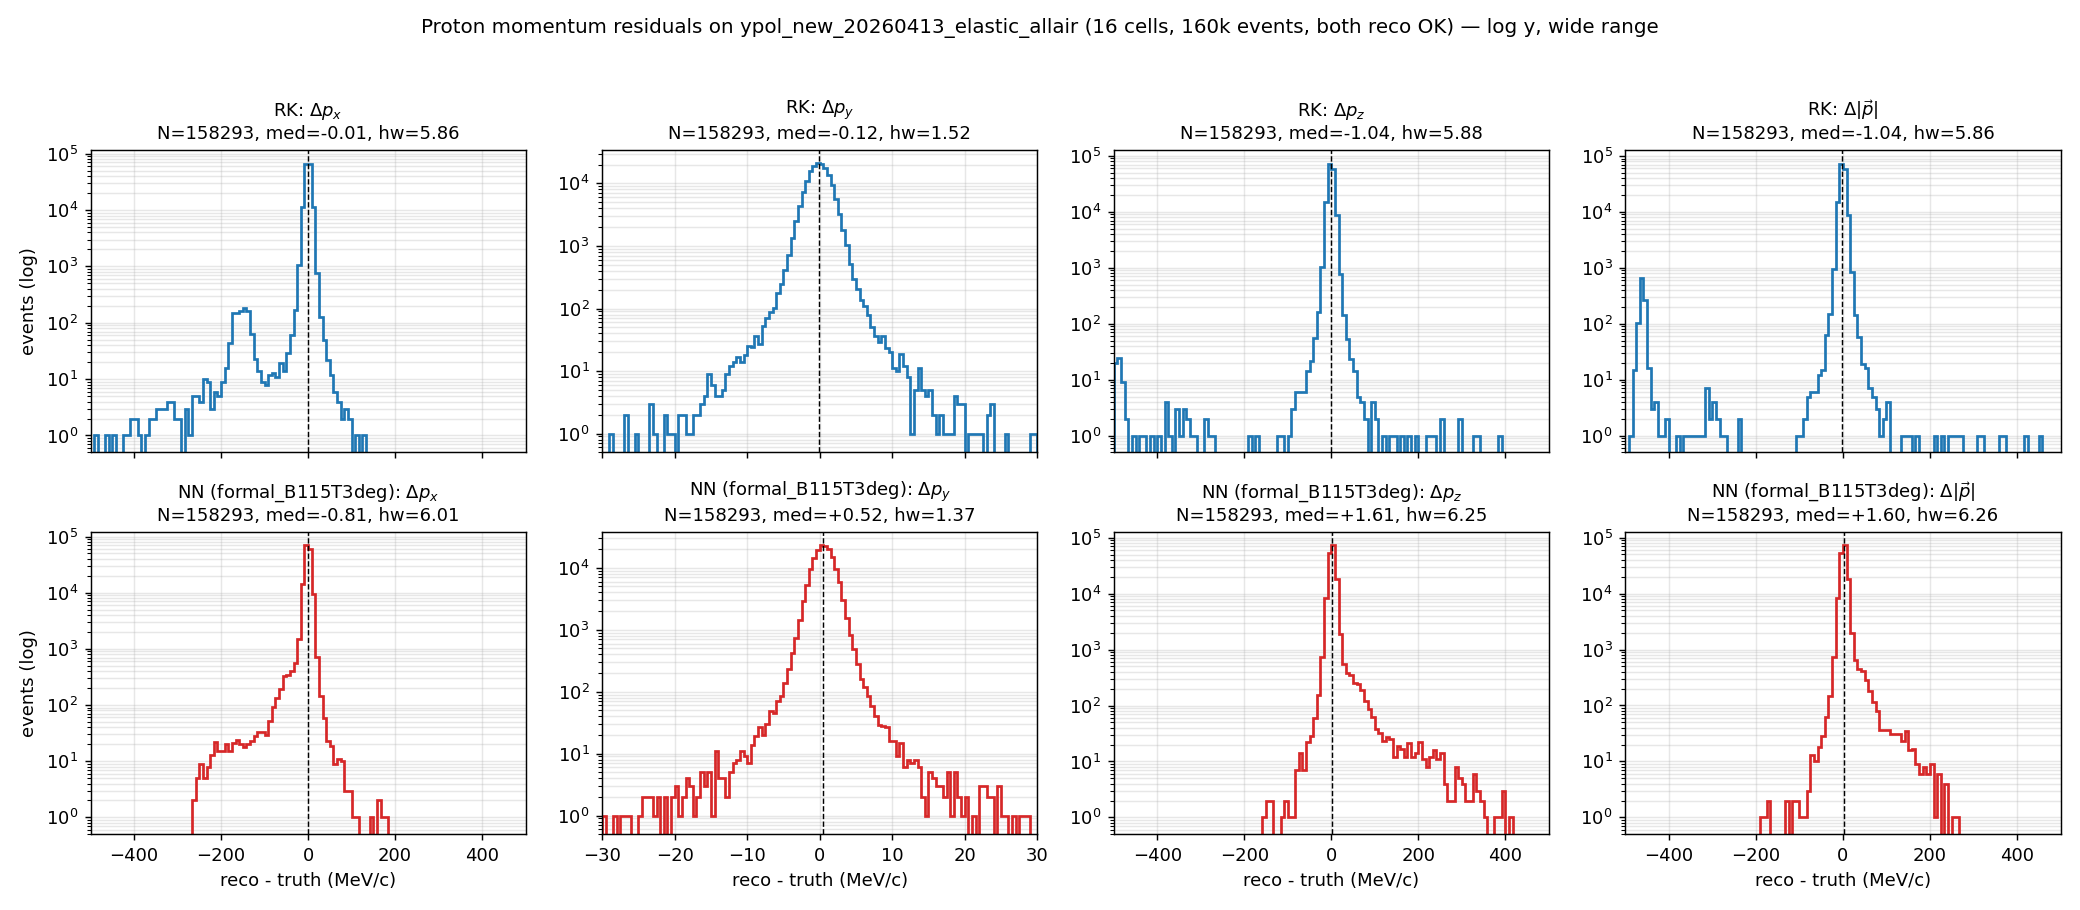
\includegraphics[width=\textwidth]{figures/ypol_phys_nn_vs_rk/residuals_grid_tail.png}
\caption{Reco $-$ truth residual distributions (158\,293-event pool, log y, wide x). Top row: RK (blue), bottom row: NN (red). Columns left to right: $\Delta p_x$, $\Delta p_y$, $\Delta p_z$, $\Delta |\vec p|$. Black dashed line = median; subplot title gives N, median, half-width. The log-y wide view exposes the RK catastrophic-failure mode in $\Delta p_x, \Delta p_z, \Delta|\vec p|$ that reaches several hundred MeV/$c$.}
\end{figure}

\begin{figure}[H]
\centering
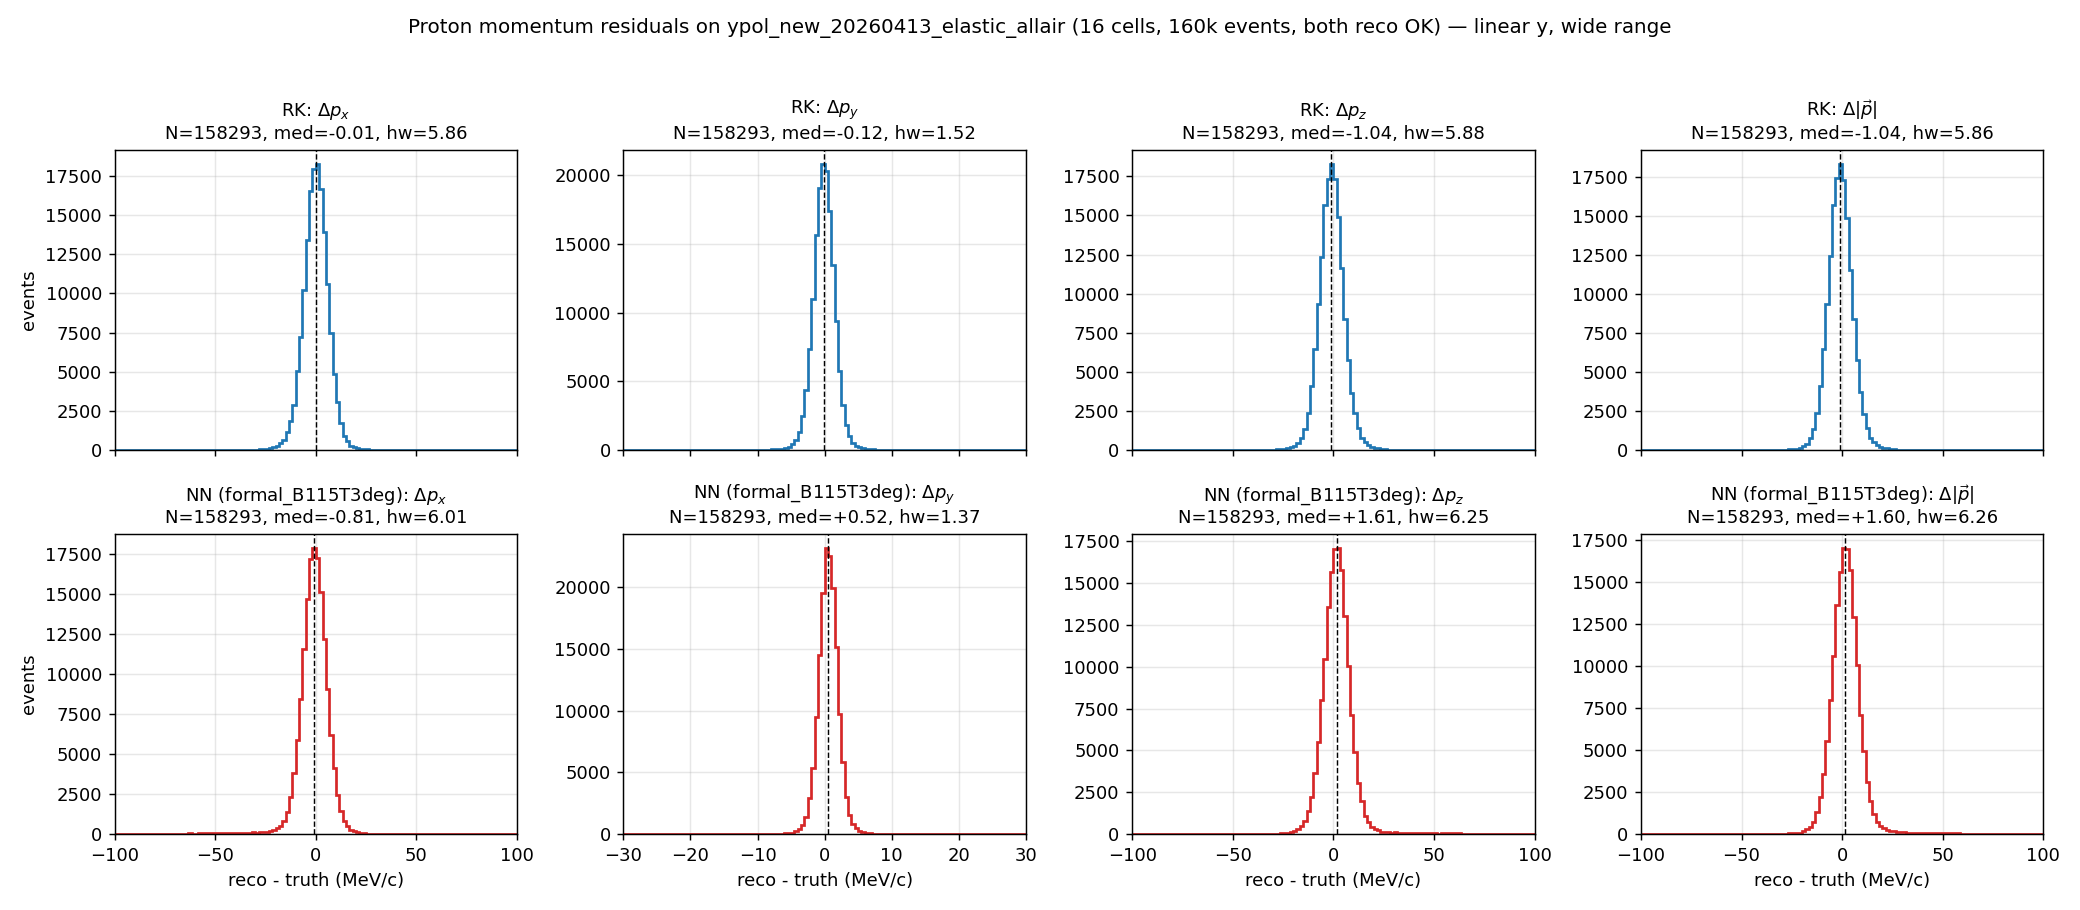
\includegraphics[width=\textwidth]{figures/ypol_phys_nn_vs_rk/residuals_grid_tail_linear.png}
\caption{Same as above, but with linear y. Same 158\,293-event pool, same wide x range. Linear y gives an intuitive comparison of central peak heights (RK and NN are within a factor of $\sim$1, comparable). RK's far tail almost touches the x-axis under linear y; the log-y view above is more useful for quantifying the tail.}
\end{figure}

\begin{figure}[H]
\centering
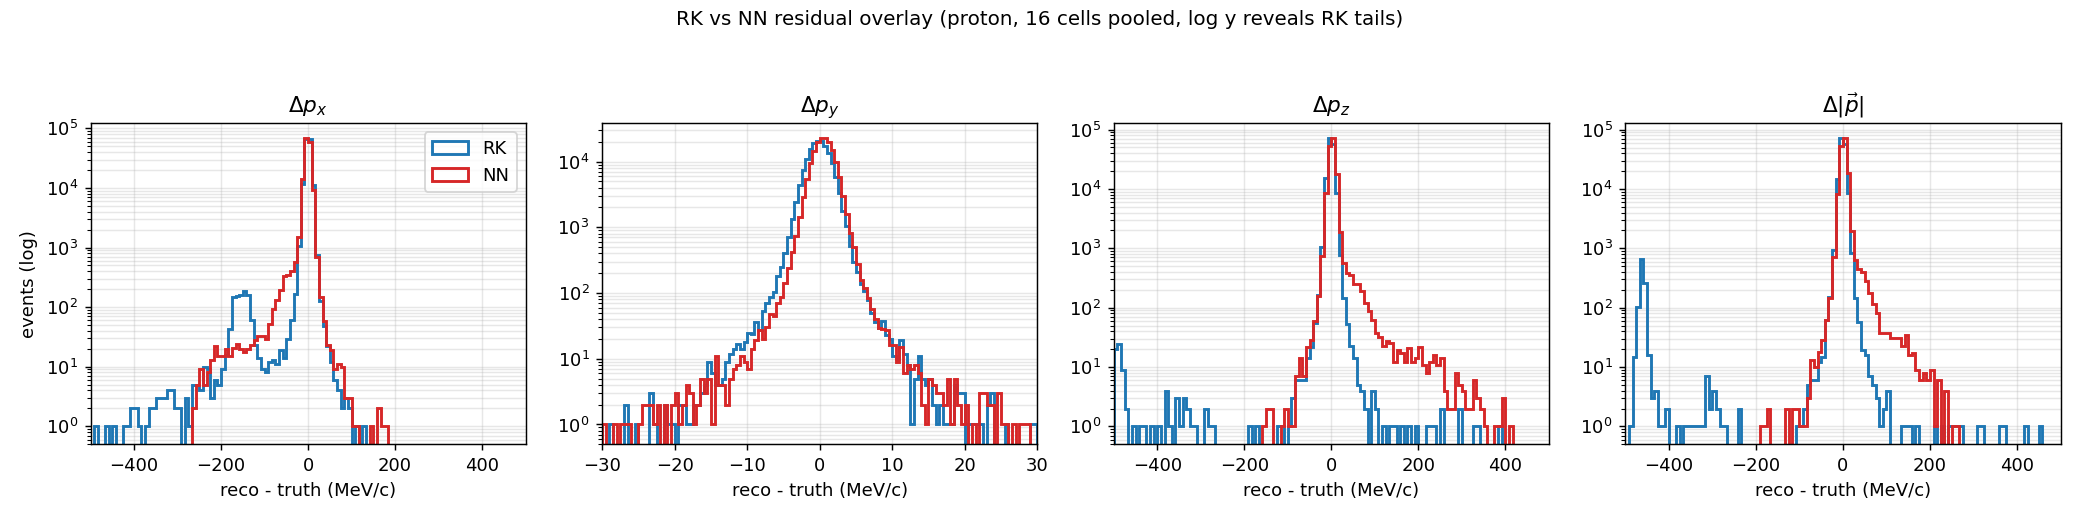
\includegraphics[width=\textwidth]{figures/ypol_phys_nn_vs_rk/residuals_overlay_tail.png}
\caption{Per-component overlay of RK (blue) and NN (red) (log y, wide x). Central peaks are similar in width, but RK's $\Delta p_x, \Delta p_z, \Delta|\vec p|$ show clear non-Gaussian tails outside $\pm 30$ MeV/$c$ that NN does not.}
\end{figure}

\begin{figure}[H]
\centering
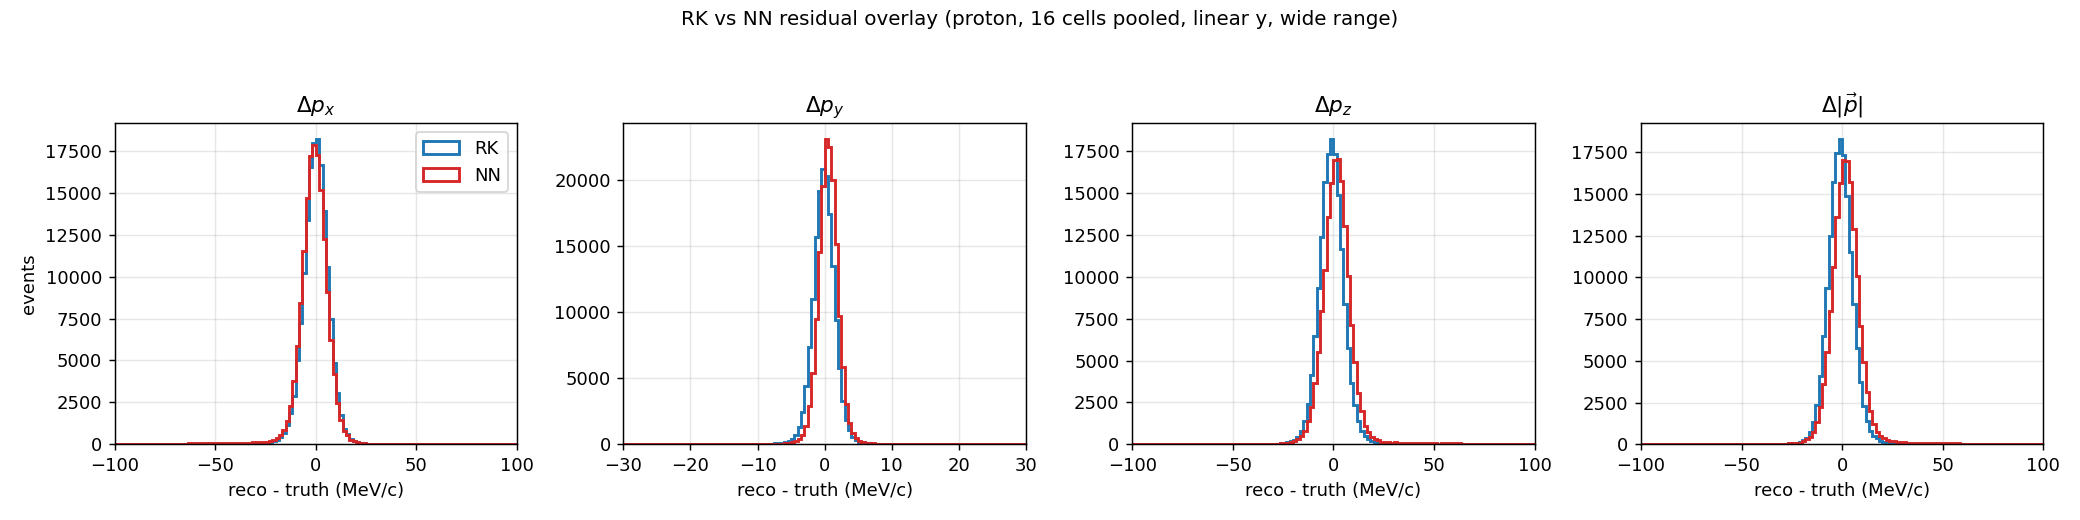
\includegraphics[width=\textwidth]{figures/ypol_phys_nn_vs_rk/residuals_overlay_tail_linear.png}
\caption{Same overlay with linear y. With central peaks aligned, RK and NN are nearly indistinguishable; the tail difference is invisible under linear y --- read together with the log-y figure above.}
\end{figure}

\subsection{3.3 reco vs truth 2D}
\begin{figure}[H]
\centering
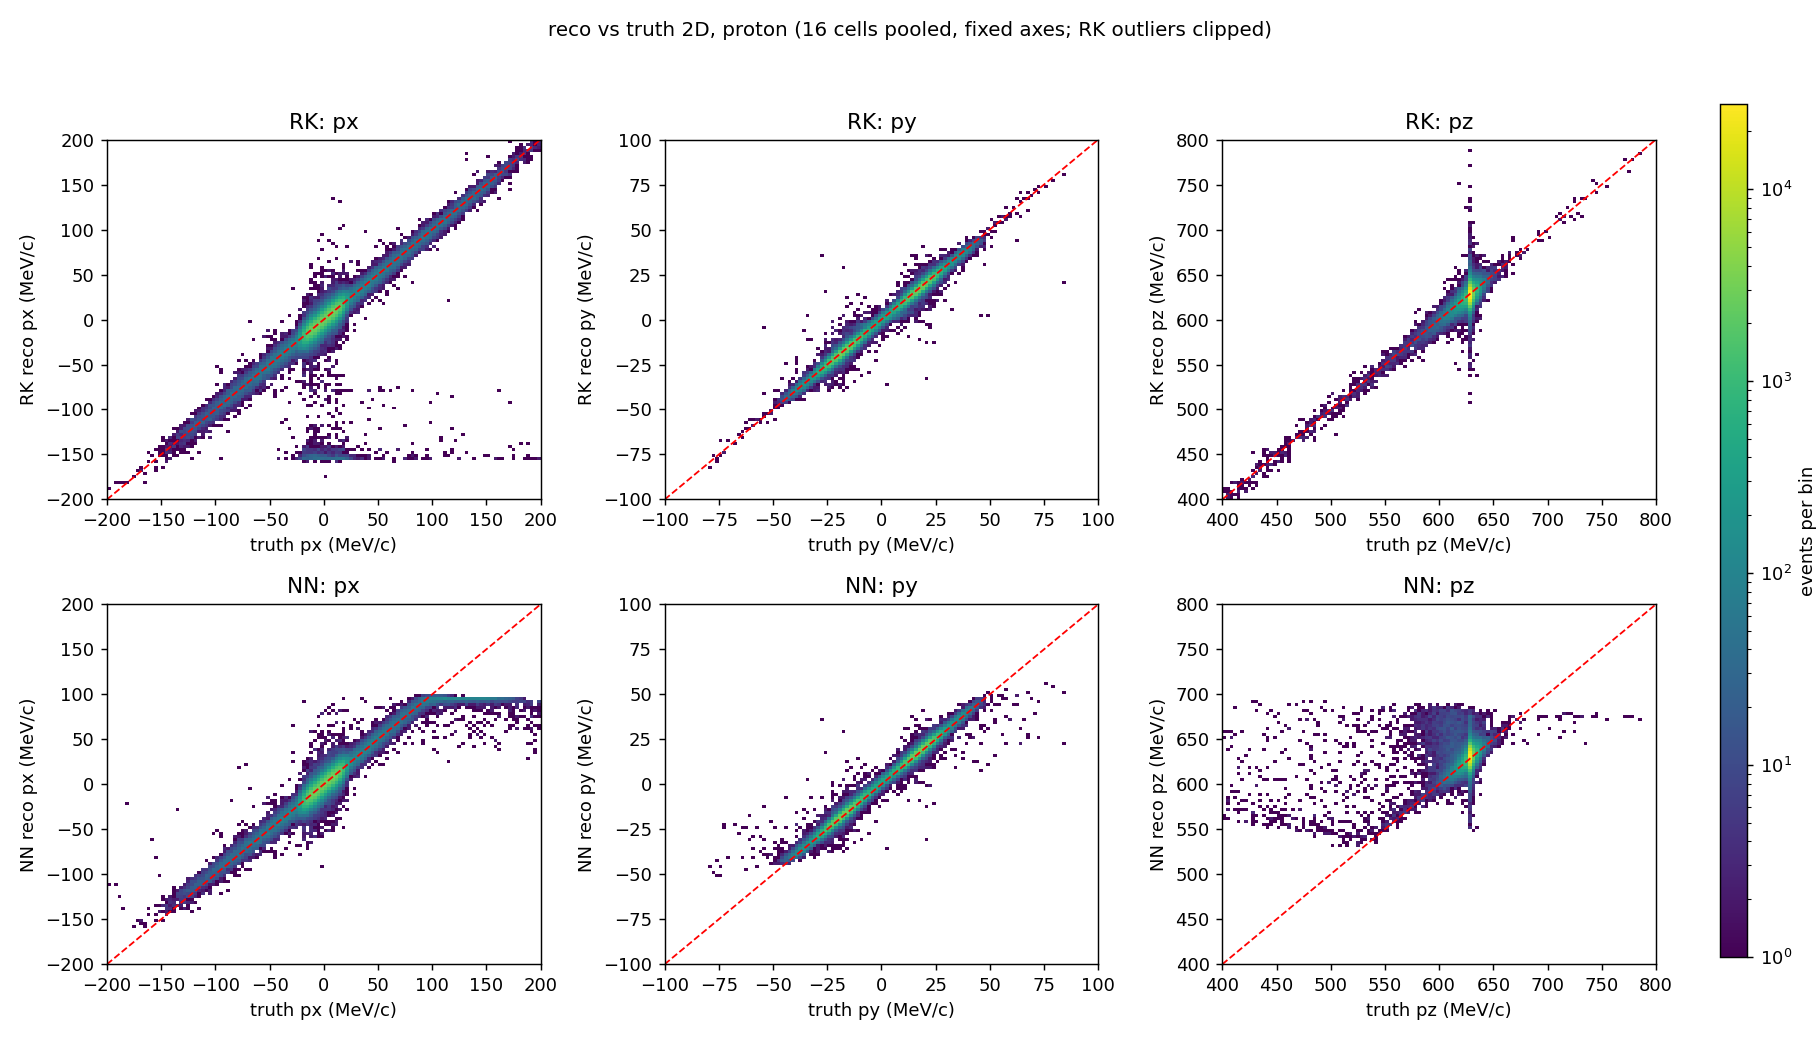
\includegraphics[width=0.95\textwidth]{figures/ypol_phys_nn_vs_rk/reco_vs_truth_2d.png}
\caption{reco vs truth 2D histograms. Top row: RK; bottom row: NN. Red dashed line $y = x$. Three columns: $p_x, p_y, p_z$. All 6 panels share a common \texttt{LogNorm} color map; the right-side colorbar gives events per bin (log scale). Both methods show the physical diagonal in $p_x$ and $p_z$; NN's diagonal is slightly wider but more symmetric, while RK has visible outliers scattering downward in $p_z$.}
\end{figure}

\section{4. Interpretation}

\subsection{4.1 Central width (1$\sigma$): essentially equivalent, NN wins on $p_y$}

NN with hidden 128/128/64 already reaches RK's analytic-reconstruction 1$\sigma$ on this near-linear PDC$\to$target geometry mapping:
\begin{itemize}[nosep]
    \item $\Delta p_x$: RK 5.86 vs NN 6.01 (NN +2.6\%), tiny gap.
    \item $\Delta p_y$: RK 1.52 vs NN \textbf{1.37} (NN $-9.9\%$, narrower). Physics-wise $p_y$ does not require solving the dipole, training data covers the regime well, and NN can use a slightly richer estimator than RK's two-point slope (implicitly leveraging PDC layer-to-layer correlations).
    \item $\Delta p_z$: RK 5.88 vs NN 6.25 (NN +6.3\%).
\end{itemize}

\subsection{4.2 Tails: NN substantially better than RK}

The most dramatic difference is the RMSE / central-width ratio:
\[
    R_\text{tail} \equiv \text{RMSE}\,/\,(\sigma_\text{eff}=\text{half-width})
\]
A pure Gaussian gives $R_\text{tail} = 1$. Measured:
\begin{table}[H]
\centering\footnotesize
\begin{tabular}{lcc}
\toprule
quantity    & RK $R_\text{tail}$ & NN $R_\text{tail}$ \\
\midrule
$\Delta p_x$    & 17.08 / 5.86 = 2.92 & 11.73 / 6.01 = 1.95 \\
$\Delta p_y$    &  1.88 / 1.52 = 1.24 &  1.82 / 1.37 = 1.33 \\
$\Delta p_z$    & 46.36 / 5.88 = 7.88 & 13.43 / 6.25 = 2.15 \\
$\Delta|\vec p|$& 39.91 / 5.86 = 6.81 & 10.77 / 6.26 = 1.72 \\
\bottomrule
\end{tabular}
\end{table}

For RK, $\Delta p_z$ and $\Delta|\vec p|$ have RMSE $\sim$\textbf{8$\times$} the 1$\sigma$ --- meaning a small fraction of events have residuals on the order of hundreds of MeV/$c$.
This matches the diagnosis in the RK report \S1.3 and \texttt{rk\_reconstruction\_status\_20260416\_zh}: dE/dx + $(u, v, p)$ linearization breaks down at low $|\vec p|$ or large angles.
NN has no such ``catastrophic'' mode: inside the training distribution, the output stays within a few tens of MeV/$c$ of truth.

\subsection{4.3 Systematic bias (median bias)}

\begin{itemize}[nosep]
    \item RK $\Delta p_x \approx 0$, $\Delta p_z = -1.04$ MeV/$c$ --- a $\sim$1 MeV/$c$ negative bias from the dE/dx model slightly underestimating energy loss between target and PDCs (already documented in RK report \S1.3).
    \item NN $\Delta p_x = -0.81$, $\Delta p_y = +0.52$, $\Delta p_z = +1.61$ MeV/$c$ --- NN has a $\sim$1 MeV/$c$ bias in \textbf{all three} directions, caused by the unweighted MSE loss + a slight mismatch between the training z-score center and the elastic-sample PDC-hit distribution. The numbers match the val biases seen at training time.
\end{itemize}

\subsection{4.4 Why is NN $\Delta p_y$ narrower than RK?}
RK's $p_y$ comes from the two-point slope of the PDC1+PDC2 y-strips: single-layer $\sim 200\,\mu$m, lever arm $\sim 1.65$ m $\to$ angular $\sigma \approx 200\,\mu\text{m}/1.65\text{m} \approx 0.12$ mrad $\to$ $\sigma(p_y) \approx 627 \times 0.12 \times 10^{-3} \approx 0.08$ MeV/$c$ (order of magnitude; multiple scattering blows it up to the 1.5 MeV/$c$ scale).
NN's input is the \textbf{full 6 coordinates} of both PDC layers, including a weak $p_y$ correlation with $(x, z)$ (second-order fringing in $y$). It learns a slightly better statistical estimator than the pure two-point slope, at the cost of a harmless $+0.5$ MeV/$c$ bias.

\section{5. Applicability and next steps}

\subsection*{5.1 Applicability}
\begin{itemize}[nosep]
    \item \textbf{Applicable}: ypol elastic-class samples ($p_z\sim 627$, $p_T\lesssim 100$ MeV/$c$), geometry fixed at \texttt{geometry\_B115T\_pdcOptimized\_20260227\_target3deg.mac}.
    \item \textbf{Use with caution}: QMD breakup / large-$p_T$ events (training domain only goes to 100 MeV/$c$). The 2.9\% of events here with $p_T > 100$ are not validated.
    \item \textbf{Domain shift}: Different geometry macro / different PDC noise $\sigma$ / different magnetic field can break the input z-score. The \texttt{run\_domain\_matched\_retrain.sh} script is for z\_pol/y\_pol domain-matched re-training, but the current secondary model (\texttt{20260228\_002757}) used only 44 training rows and has RMSE $>$ 100 MeV/$c$ --- not usable; needs full re-training.
\end{itemize}

\subsection*{5.2 Recommended use}
Based on this evaluation, in ypol-elastic-class analyses NN reconstruction \textbf{can directly replace RK}. Gains:
\begin{itemize}[nosep]
    \item Pass rate up to 100\% (RK loses $\sim$1.1\% events);
    \item RK's $|\vec p|$ catastrophic failures eliminated (RMSE down $\sim 4\times$);
    \item $p_y$ 1$\sigma$ slightly better.
\end{itemize}
Costs:
\begin{itemize}[nosep]
    \item A 1--2 MeV/$c$ bias is introduced in all three components (below 0.3\% of $|\vec p|$ in this sample, negligible for reaction-plane / R-ratio analyses).
    \item No per-event $\chi^2$ / Laplace error estimate as RK provides; harder to do per-event precision weighting.
\end{itemize}

\subsection*{5.3 Next steps (priority order)}
\begin{enumerate}[nosep]
    \item Run the same NN inference on \texttt{eval\_target3deg\_smoke\_20260228\_ypol} / \texttt{eval\_20260227\_235751} and check the impact of NN systematic bias on $\Delta R_x^\text{rot}$ (expected $<1\%$).
    \item Train a ``wide-window'' model with $R = 200$ disk + $p_z\in[400, 800]$ to cover QMD breakup; re-evaluate on ypol elastic to check for regression.
    \item Add a heteroscedastic uncertainty head next to the NN output for downstream $\chi^2$ weighting.
\end{enumerate}

\section*{Artifacts}
\begin{itemize}[nosep]
    \item NN reco output: \texttt{build/test\_output/ypol\_phys\_20260428/reco\_nn/<tag>\_reco\_nn.root}
    \item Extraction macro: \texttt{scripts/analysis/ypol\_phys/extract\_proton\_rk\_nn.C}
    \item Residual analysis: \texttt{scripts/analysis/ypol\_phys/analyze\_nn\_vs\_rk\_residuals.py}
    \item Per-cell CSV: \texttt{build/test\_output/ypol\_phys\_20260428/csv\_rk\_nn/}
    \item Residual summaries: \texttt{docs/reports/reconstruction/momentum\_reco/nn/figures/ypol\_phys\_nn\_vs\_rk/summary.\{json,txt\}}
    \item Per-cell table: \texttt{per\_cell\_summary.csv} in the same directory.
\end{itemize}

\end{document}
